% **************************************************************************
% System design 
% **************************************************************************

\chapter{Title of chapter 2}


% ---------------------------------------------------------------------------
  \begin{center}
  \textbf{\LARGE Abstract}
  \end{center}

  This chapter considers SOMETHING.
  %
  We show that...

\clearpage

% ---------------------------------------------------------------------------
\section{Introduction} 

In this chapter, we focus on SOMETHING

%-----------------------------------------------
\subsection{Network Model}\label{comm-ssec:model}
%-----------------------------------------------


In addition,~\cite{alasfour2018coarse} demonstrates that from such data, behavior-specific contexts can be discriminated from freely recorded neural activity.

Here is a figure:
\begin{figure}[!ht]
\centering
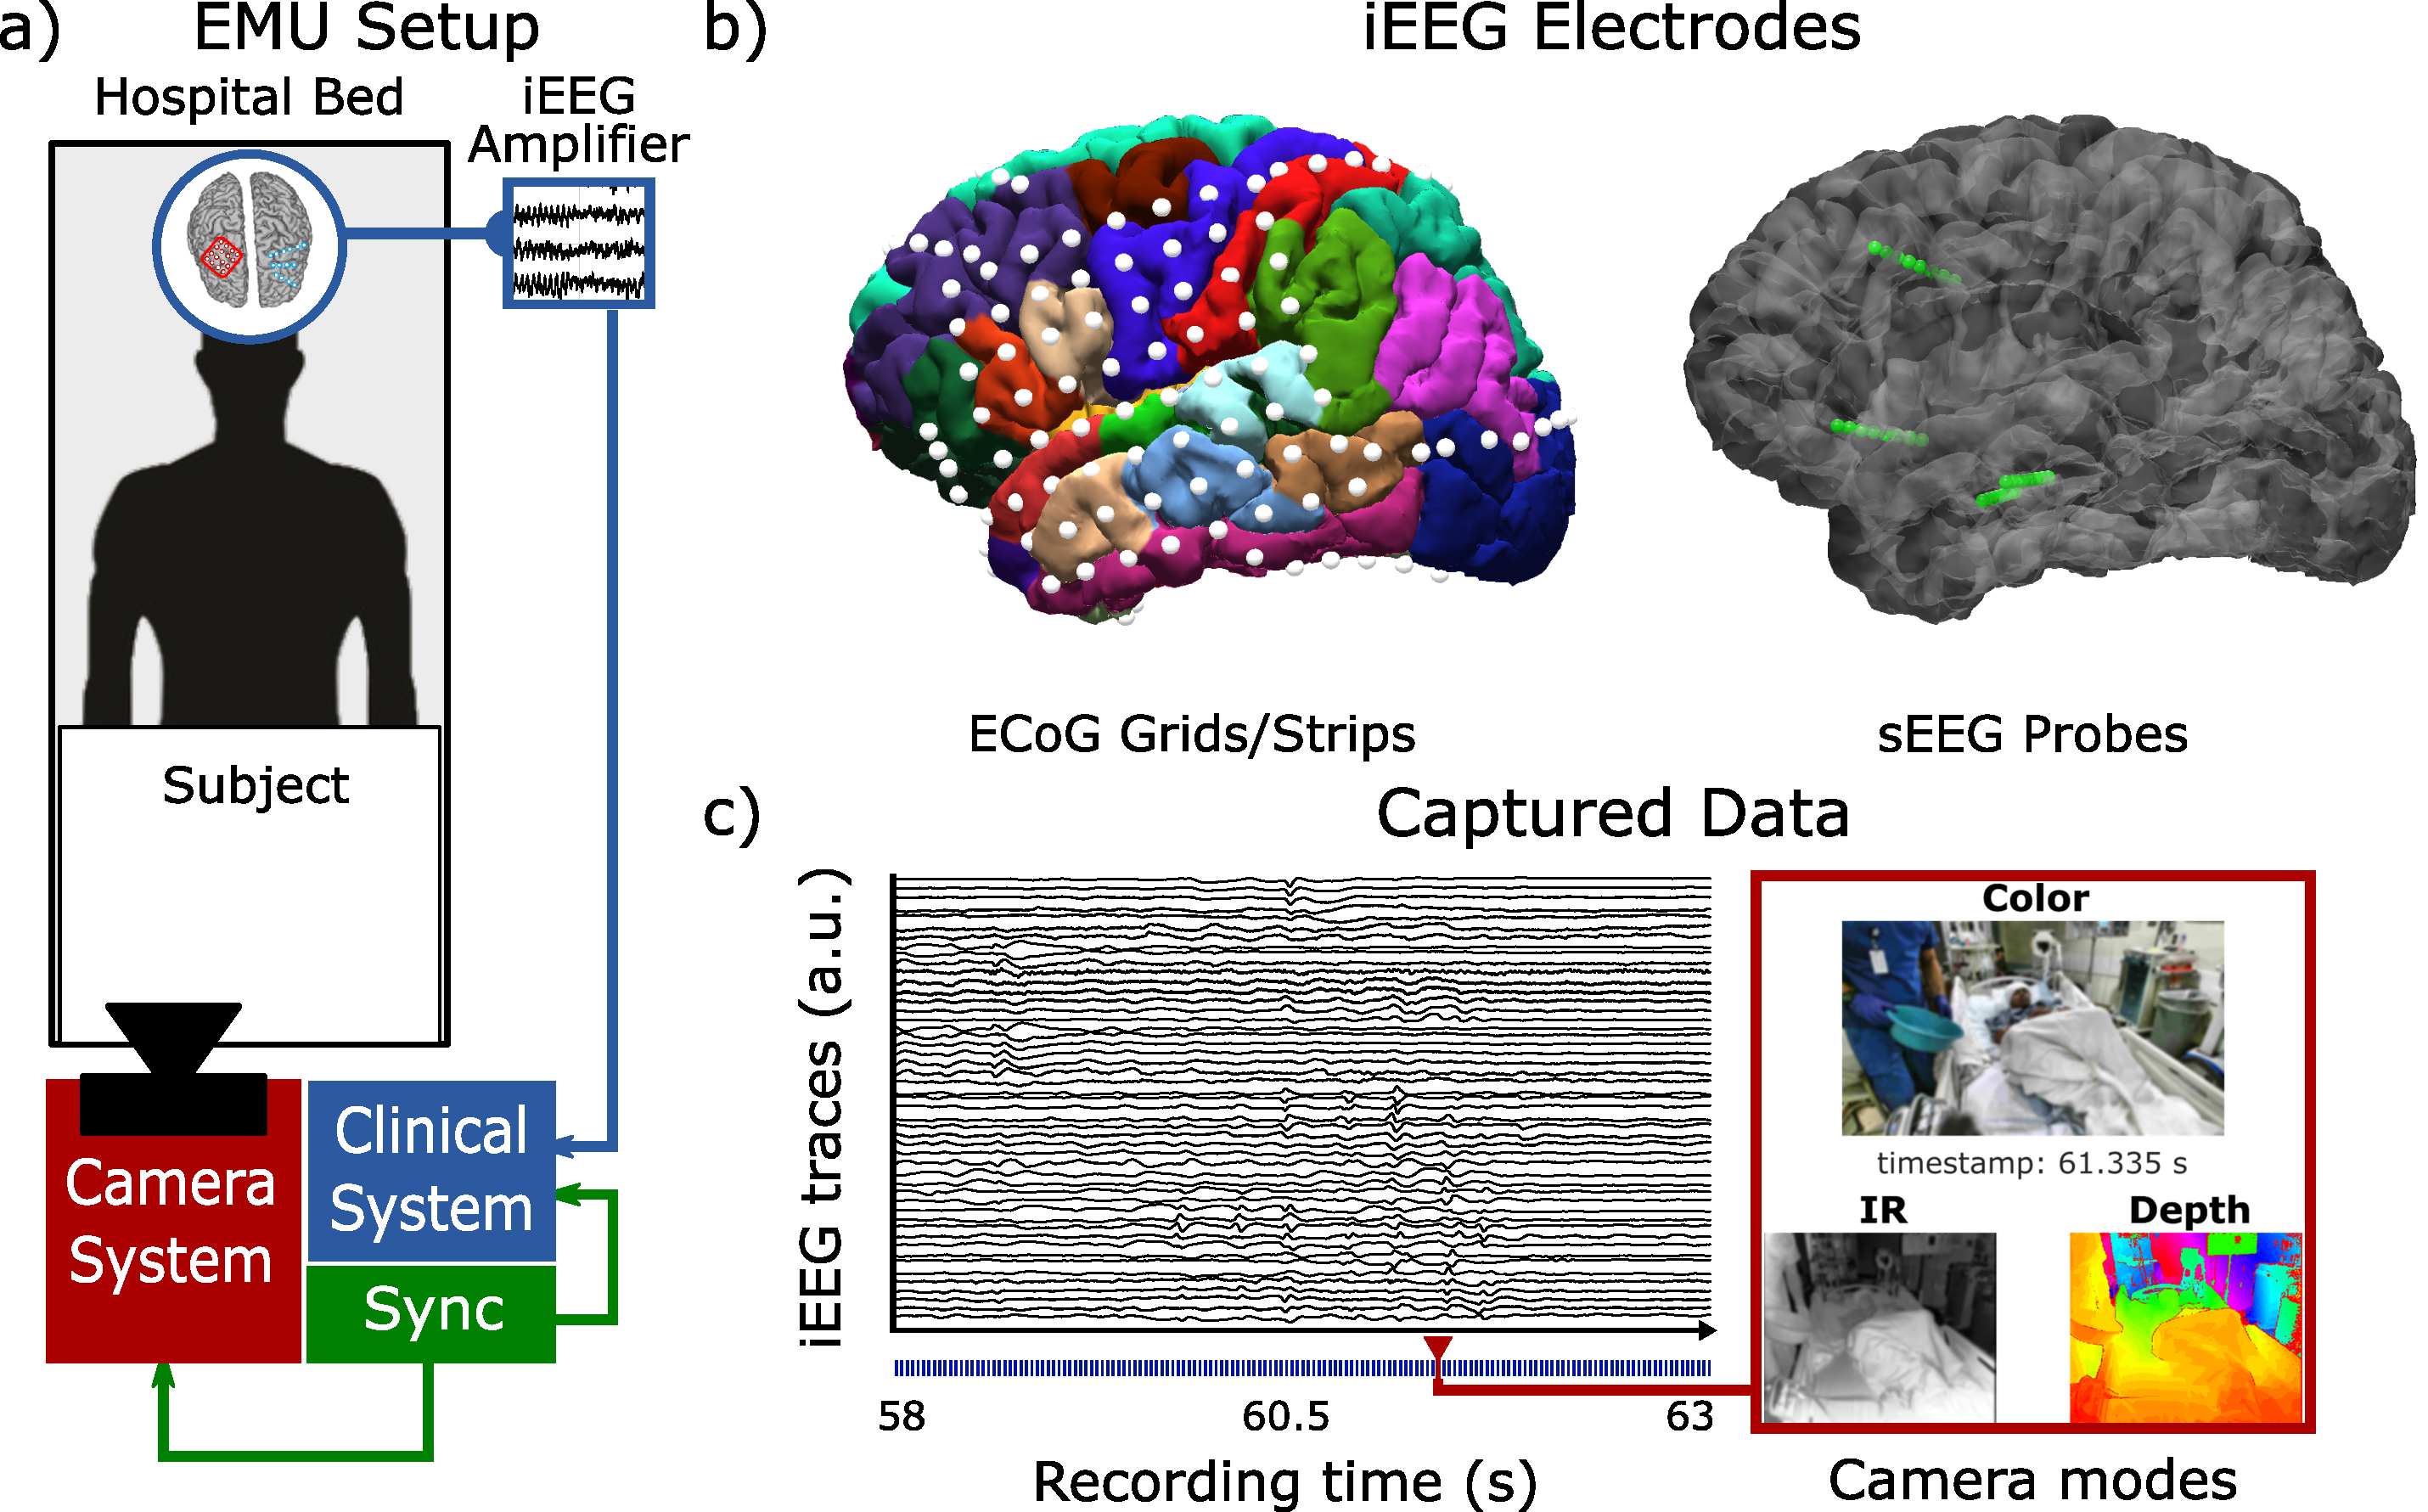
\includegraphics[width=0.85\textwidth]{img/method_setup.pdf}
\caption[This is the short form of the caption. It has to be no more than 4 lines.]{\textbf{Diagram of experimental setup for recording behavioral video simultaneously with intracortical activity (ECoG, sEEG) from subjects in the epilepsy monitoring unit.} \textbf{a)} The experimental setup places the video recording system at the foot of the hospital bed facing the subject to capture the subject and their immediate surroundings. \textbf{b)} A typical subject has over 100 electrodes placed according to clinical need, as shown in the reconstructed coverage of ECoG and sEEG for Subject 1. A combination of subdural grid and strip electrodes (ECoG) covers many regions of the cortical surface, depicted by the Desikan-Killiany parcellation~\cite{desikan2006automated}, while stereotactic depth probes (sEEG) sample deep and superficial brain structures. \textbf{c)} During the study, videos (blue) of the subject moving in an uninstructed and unstructured manner are captured using a Kinect for Windows (v2) sensor. An example of the sensor modalities is framed in red. A subset of 50 neural traces recorded in parallel shown underneath, aligned $\leq 5ms$ of each video frame. Data collected in this manner captures an external and intracortical representation of each subject's movement. A preliminary demonstration using neural features in relation to movement segments marked using only the color video stream is detailed in this work.}
\label{fig-setup}
\end{figure}

%-------------------------------------
\subsection{Related Work} \label{comm-ssec:previous_work}
%-------------------------------------
Text

%------------------------------------------
\subsection{Our Contributions}\label{comm-ssec:contributions}
%------------------------------------------
Text

\clearpage

%-------------------------------------------------------

%------------------------------------------------
\section{Open Questions}
\label{comm-sec:conclusions}

% % Chapter Bibliography
\clearpage
\bibliographystyle{unsrt}
\bibliography{bib}

% \vfill

% \noindent\rule[0.5ex]{\linewidth}{1pt}

% % Include citation if chapter is published

% This chapter
% is a reprint of the material as it appears in
% SOURCE
% %
% The dissertation author was the primary investigator of this paper.
% %
% \copyright{} IEEE. 
% Reprinted with 
% permission.
